\documentclass{beamer}

\usetheme{Warsaw}
\definecolor{indigo(web)}{rgb}{0.29, 0.0, 0.51}
\usecolortheme[named=indigo(web)]{structure}

% used for lines in tables
\usepackage{booktabs}


% package for including source code
% https://en.wikibooks.org/wiki/LaTeX/Source_Code_Listings
% http://mirrors.fe.up.pt/pub/CTAN/macros/latex/contrib/listings/listings.pdf
\usepackage{listings}

% package for drawings
\usepackage{tikz}
\usetikzlibrary{trees}

\title[Improving reproducibility in building simulation]{Improving reproducibility in building simulation: a pure-Python approach to geometry creation}
\author{Steven Firth}
\institute{Loughborough University}
\date{2021-06-23}

\begin{document}
	
	\begin{frame}
		\maketitle
	\end{frame}
	
	\begin{frame}{My background}
		\begin{itemize}
			\item I joined Loughborough University in 2008
			\item My job title is Reader in Building Performance Modelling
			\item I teach building simulation, energy data analysis, sustainable building design and renewable energy.
			\item I was a member of the University's Open Research Working Group in 2019.
			\item I was awarded the CALIBRE Winter 2019 Award for Open Research
			\item In 2015 I published the Refit Smart Home dataset on the University's Data Repository (14,307 views, 3,997 downloads)
			\item I publish papers on FAIR data and open research methods using Python and Jupyter Notebooks 
			\item I maintain the GitHub pages for the Building Energy Research Group
			
		\end{itemize}
	\end{frame}

	\begin{frame}{Point-and-click vs. Text-based commands}
		\hyphenpenalty=100000
		\begin{tabular}{p{0.3\textwidth}p{0.3\textwidth}p{0.3\textwidth}}
			\toprule
			Research task & Point-and-Click & Text-based Commands \\
			\midrule
			Writing documents & Microsoft Word & \LaTeX \\
			Creating slides & Microsoft PowerPoint & \LaTeX \\
			Analysing data & Microsoft Excel & Python and Jupyter Notebooks \\
			Building websites & Adobe Dreamweaver & HTML, Bootstrap, Django
		\end{tabular}
	\end{frame}

	\begin{frame}{Example \#1: A Reproducible Presentation}
		This presentation is reproducible as it is written in code (Latex)\\[10pt]
		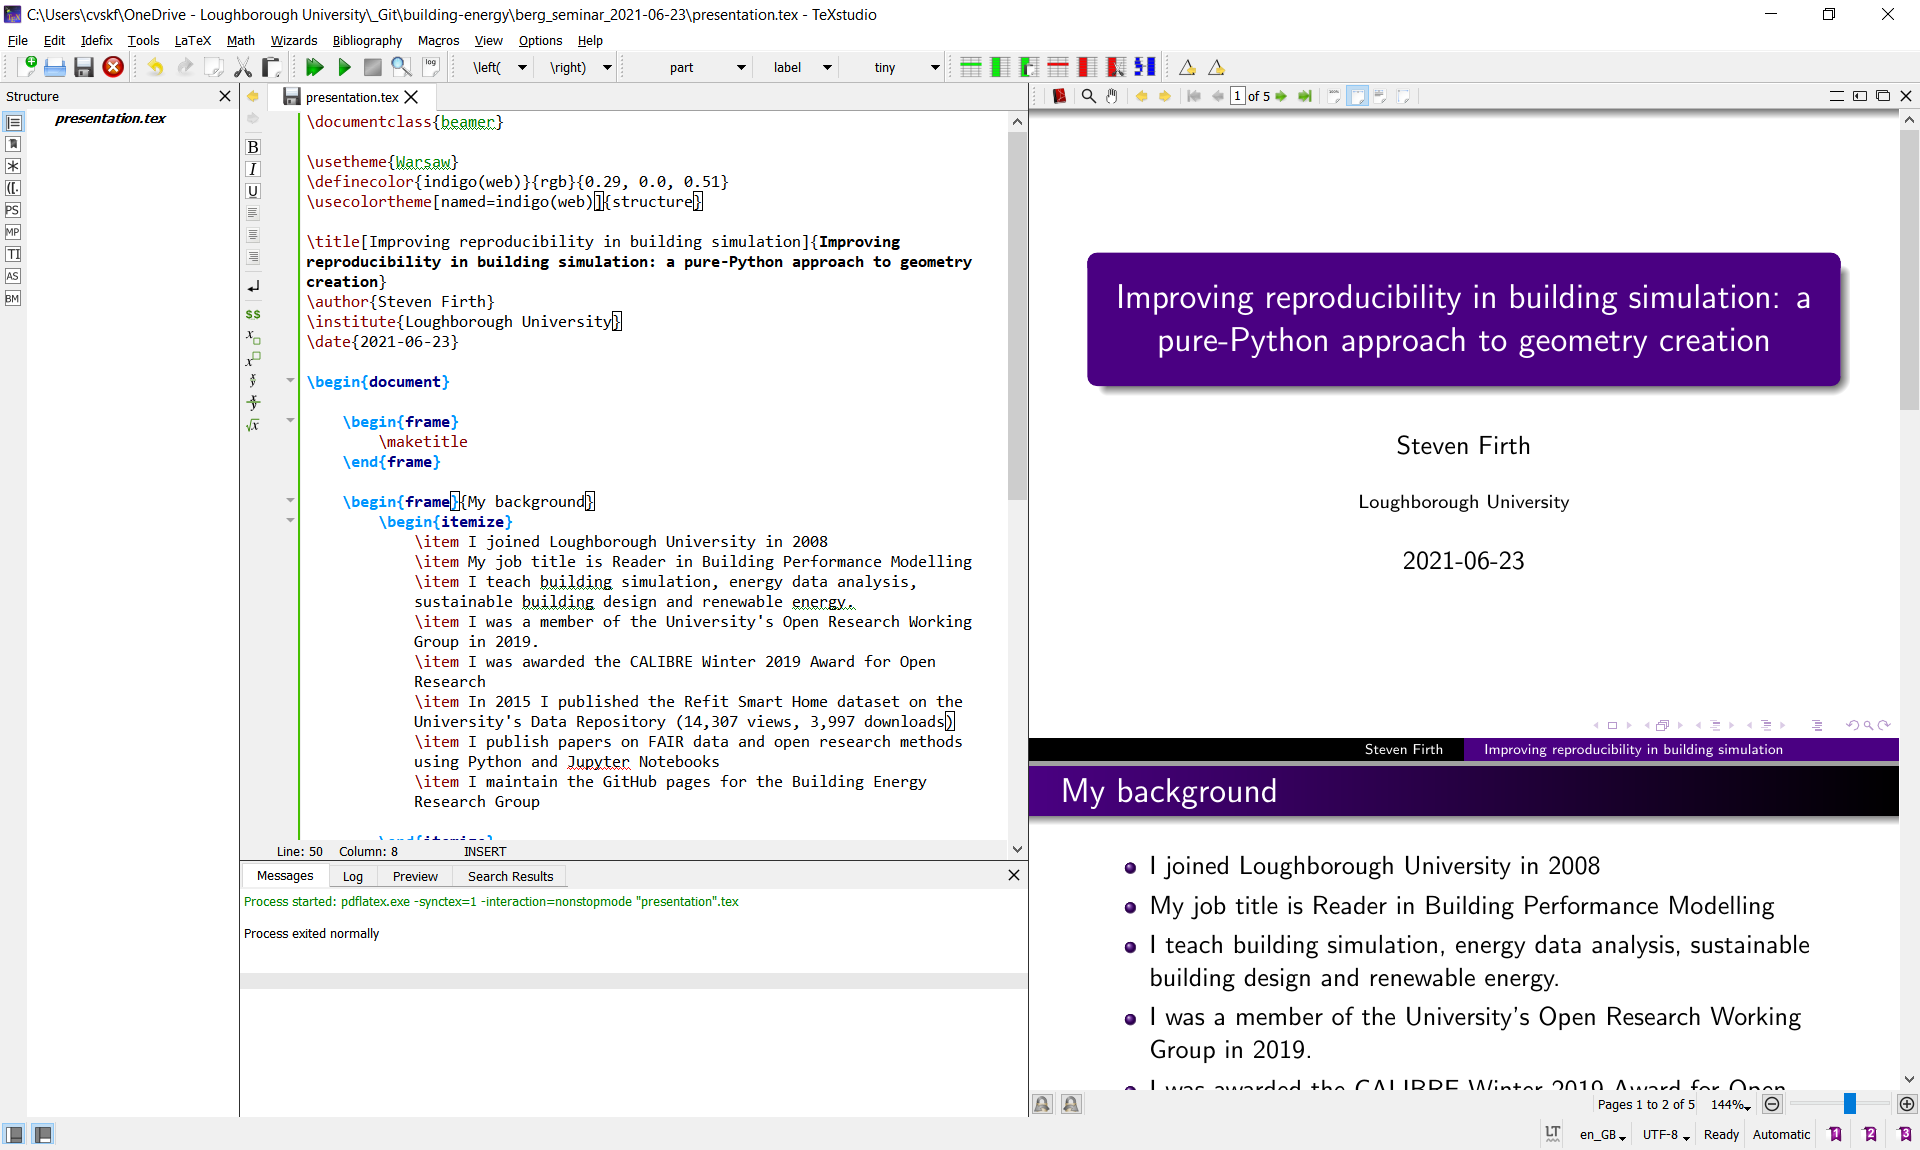
\includegraphics[width=\textwidth,keepaspectratio]{latex_example.png}
	\end{frame}
	
	\begin{frame}{Example \#1: A Reproducible Presentation}
		This presentation is also open as the code is hosted on the BERG Github repository\\[10pt]
		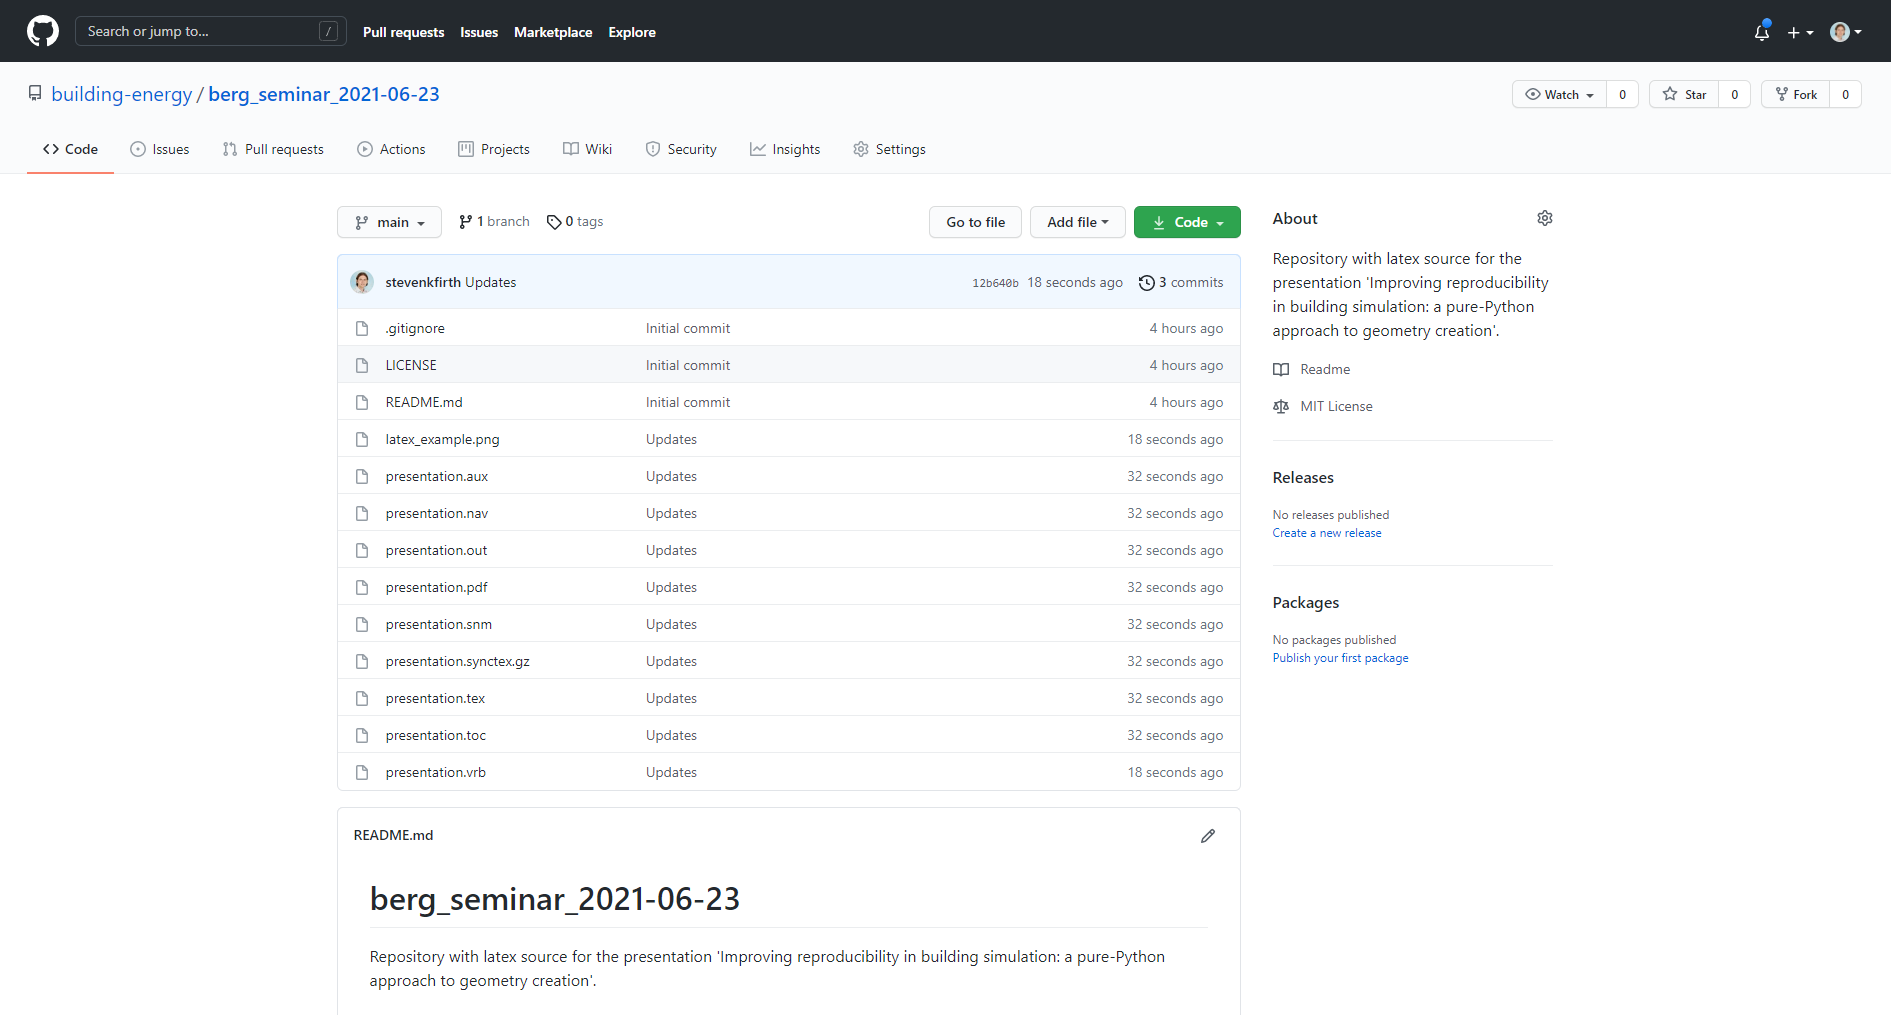
\includegraphics[width=\textwidth,keepaspectratio]{github_example.png}
	\end{frame}

	\begin{frame}{The problem I am trying to solve}
		\begin{itemize}
			\Large
			\item \textbf{Task:} I would like \emph{to construct a building simulation model} of a building and \emph{to simulate the energy performance} of the building using the EnergyPlus software.\\[10pt]
			\item \textbf{Challenge:} I would like to do this in an \emph{open, transparent} way so that the whole process is \emph{reproducible}. 
		\end{itemize}
	\end{frame}

	\begin{frame}{I'm going to do this in Python}
	
		Python is one of the world's best known computer languages.\\[10pt]
		
		Specifically designed to be easy for others to read - this enhances \textit{reproducibility}.\\[10pt]
		
		The language of choice for the building simulation community.
		\begin{itemize}
			\item EnergyPlus has a Python plug-in.
			\item Building simulation software such as IES and DesignBuilder allow Python scripting.
			\item The eSIM 2021 conference accepted submissions of Jupyter Notebooks written in Python.
		\end{itemize}
		
		\vspace{5pt}
		
		\centering
		
\includegraphics[width=0.5\textwidth,keepaspectratio]{python-logo-master-v3-TM.png}
		
	\end{frame}


	\begin{frame}{I'm going to develop Python packages}

		Python packages are libraries of reusable code.
		\begin{itemize}
			\item They have an API which exposes classes and functions.
			\item The classes provide object instances which can store data and class methods.
		\end{itemize}

		\vspace{10pt}

		Well-known examples of Python packages are:
		\begin{itemize}
			\item \textit{pandas} $\rightarrow$ data analysis
			\item \textit{matplotlib} $\rightarrow$ plotting graphs and figures
		\end{itemize}
	
		\vspace{10pt}
	
		Packages can be hosted on \textit{GitHub} $\rightarrow$ allows others to contribute $\rightarrow$ open source software.

	\end{frame}

	\begin{frame}{Example \#2: the SAP2012 package}
		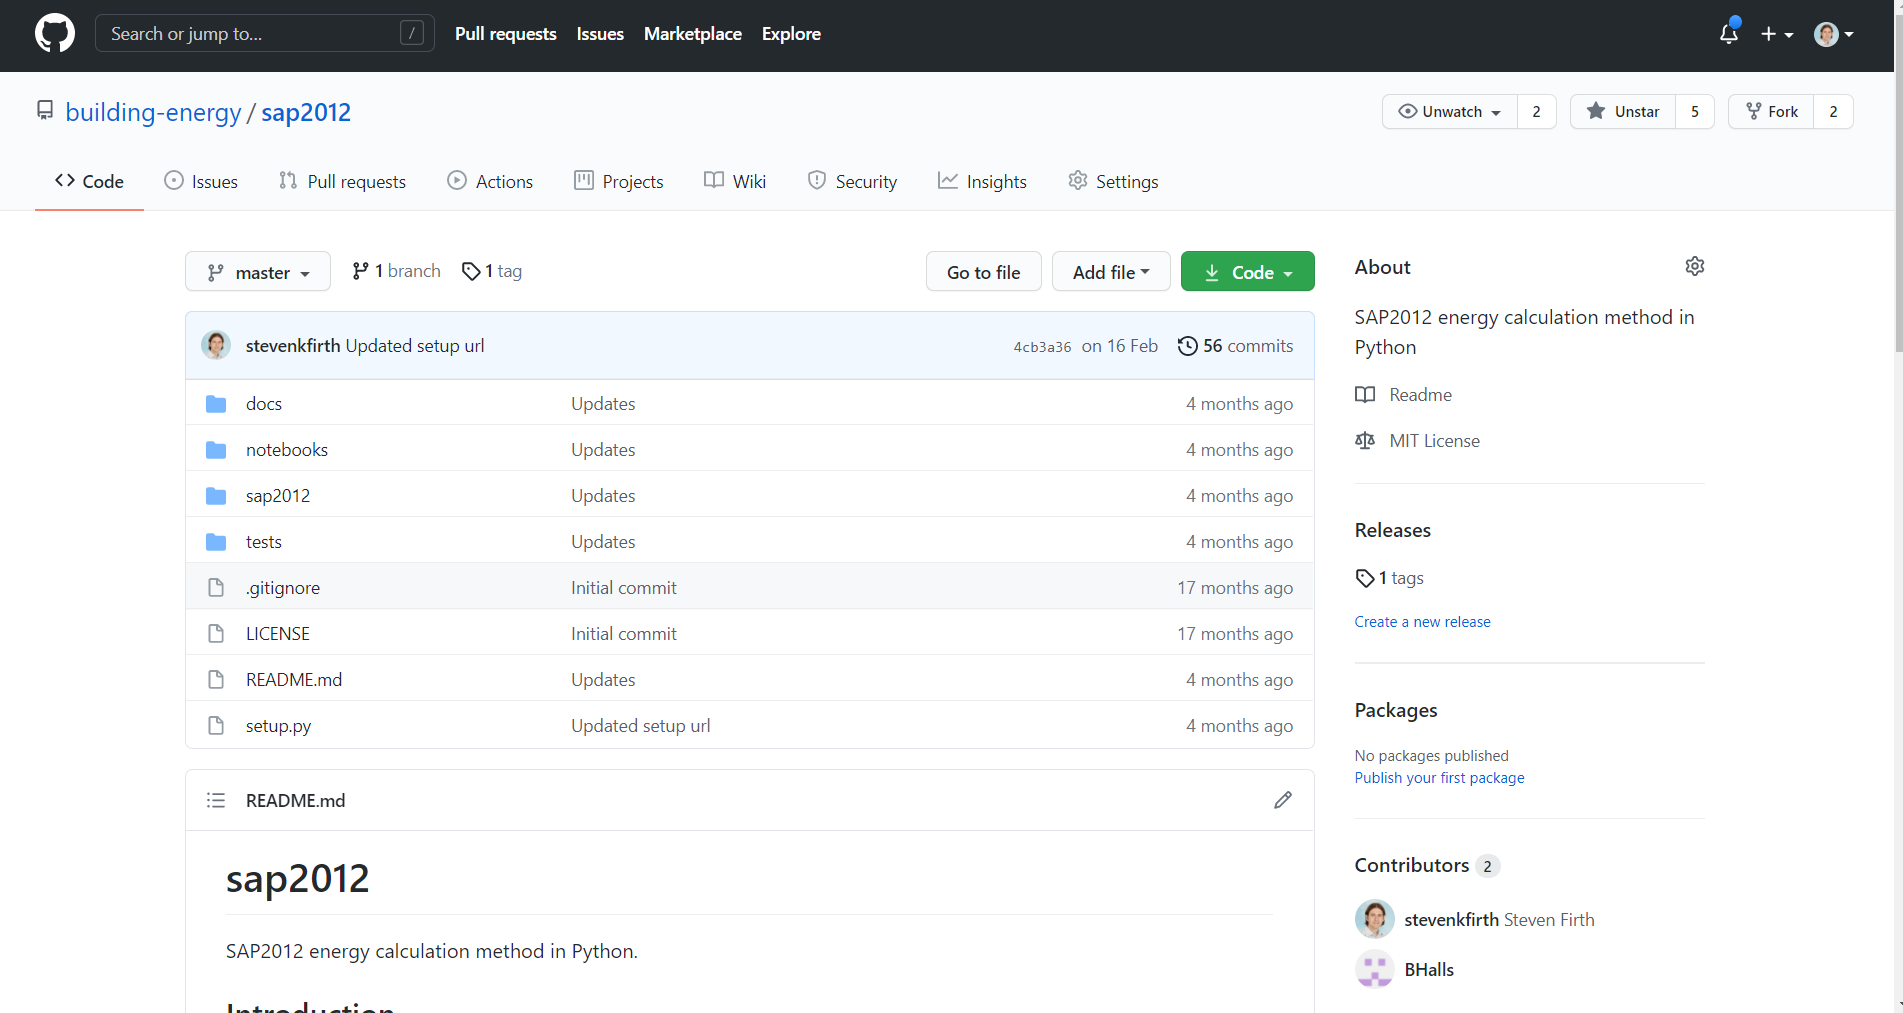
\includegraphics[width=1\textwidth,keepaspectratio]{github_sap_2012.png}
	\end{frame}

	\begin{frame}{Example \#2: the SAP2012 package}
		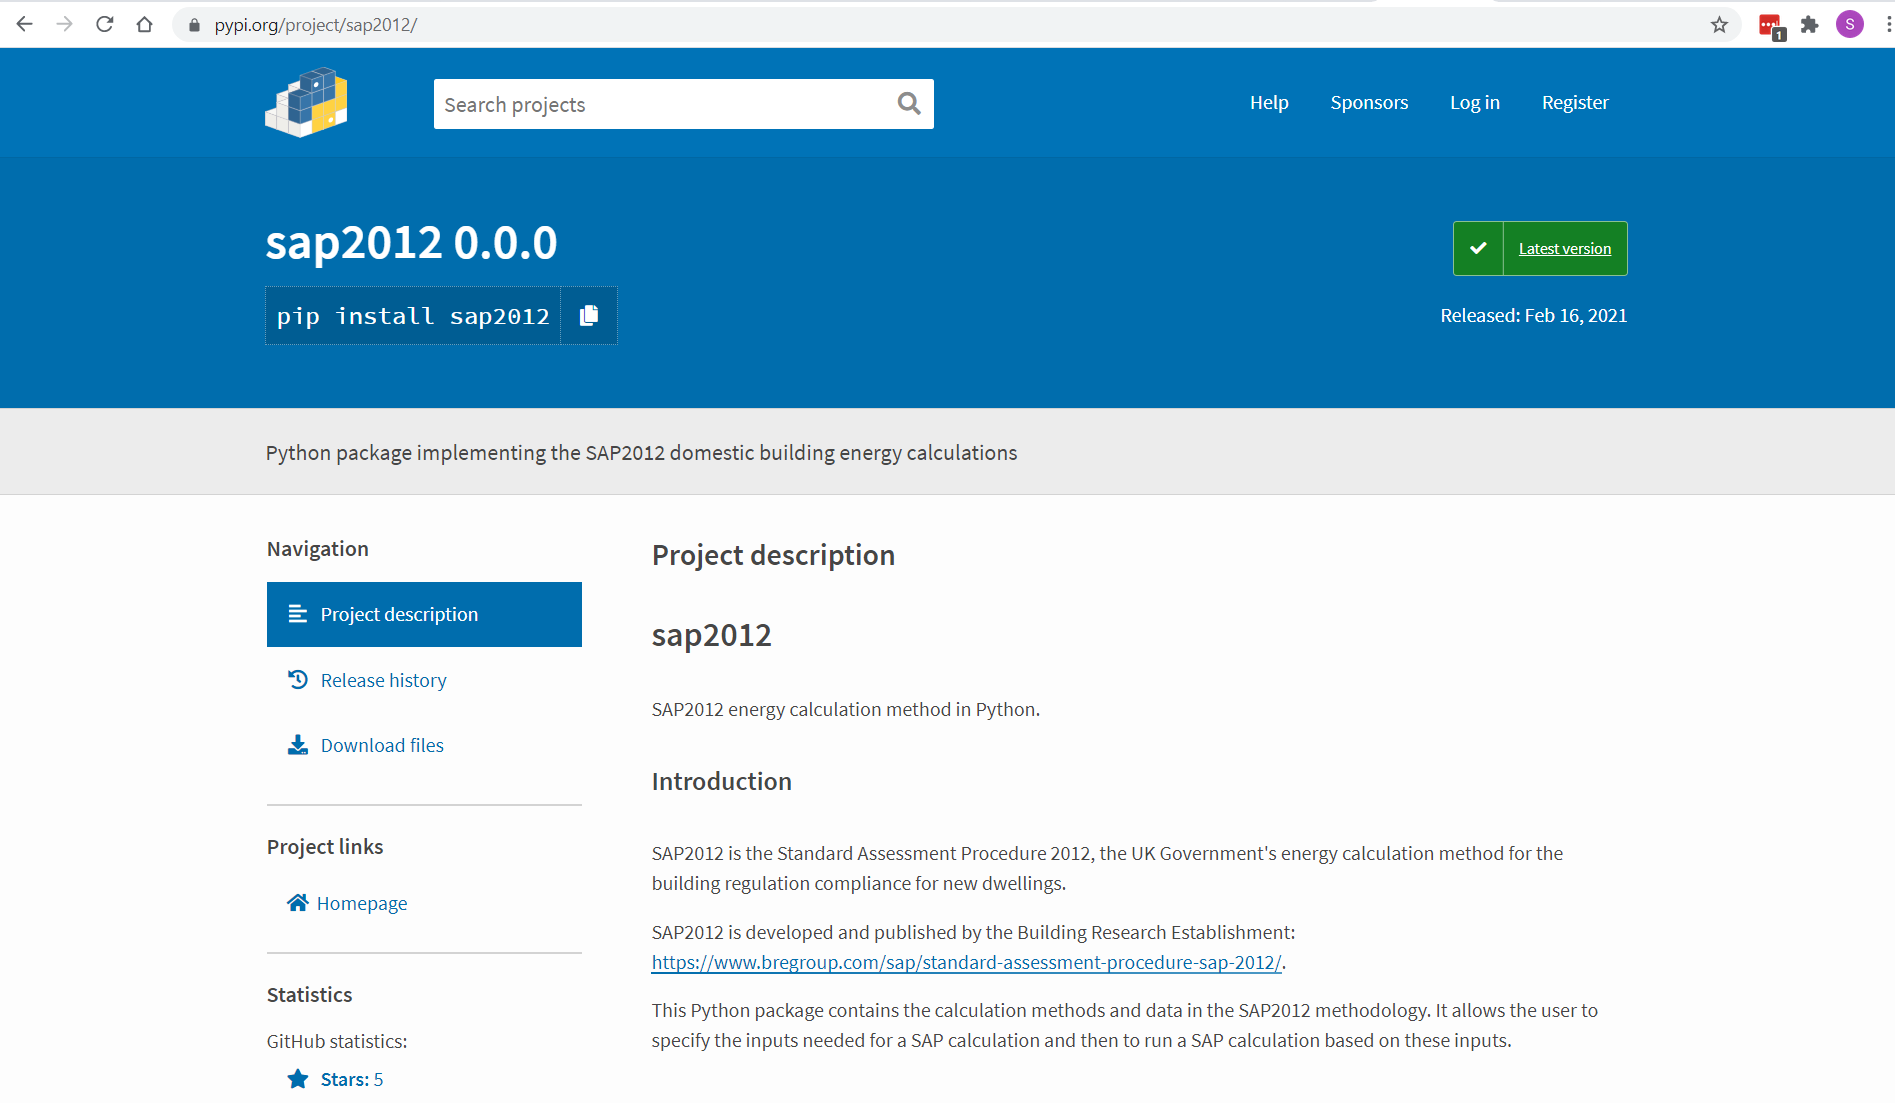
\includegraphics[width=1\textwidth,keepaspectratio]{pypi_sap_2012.png}
	\end{frame}

	\begin{frame}{Example \#2: the SAP2012 package}
		\begin{figure}
			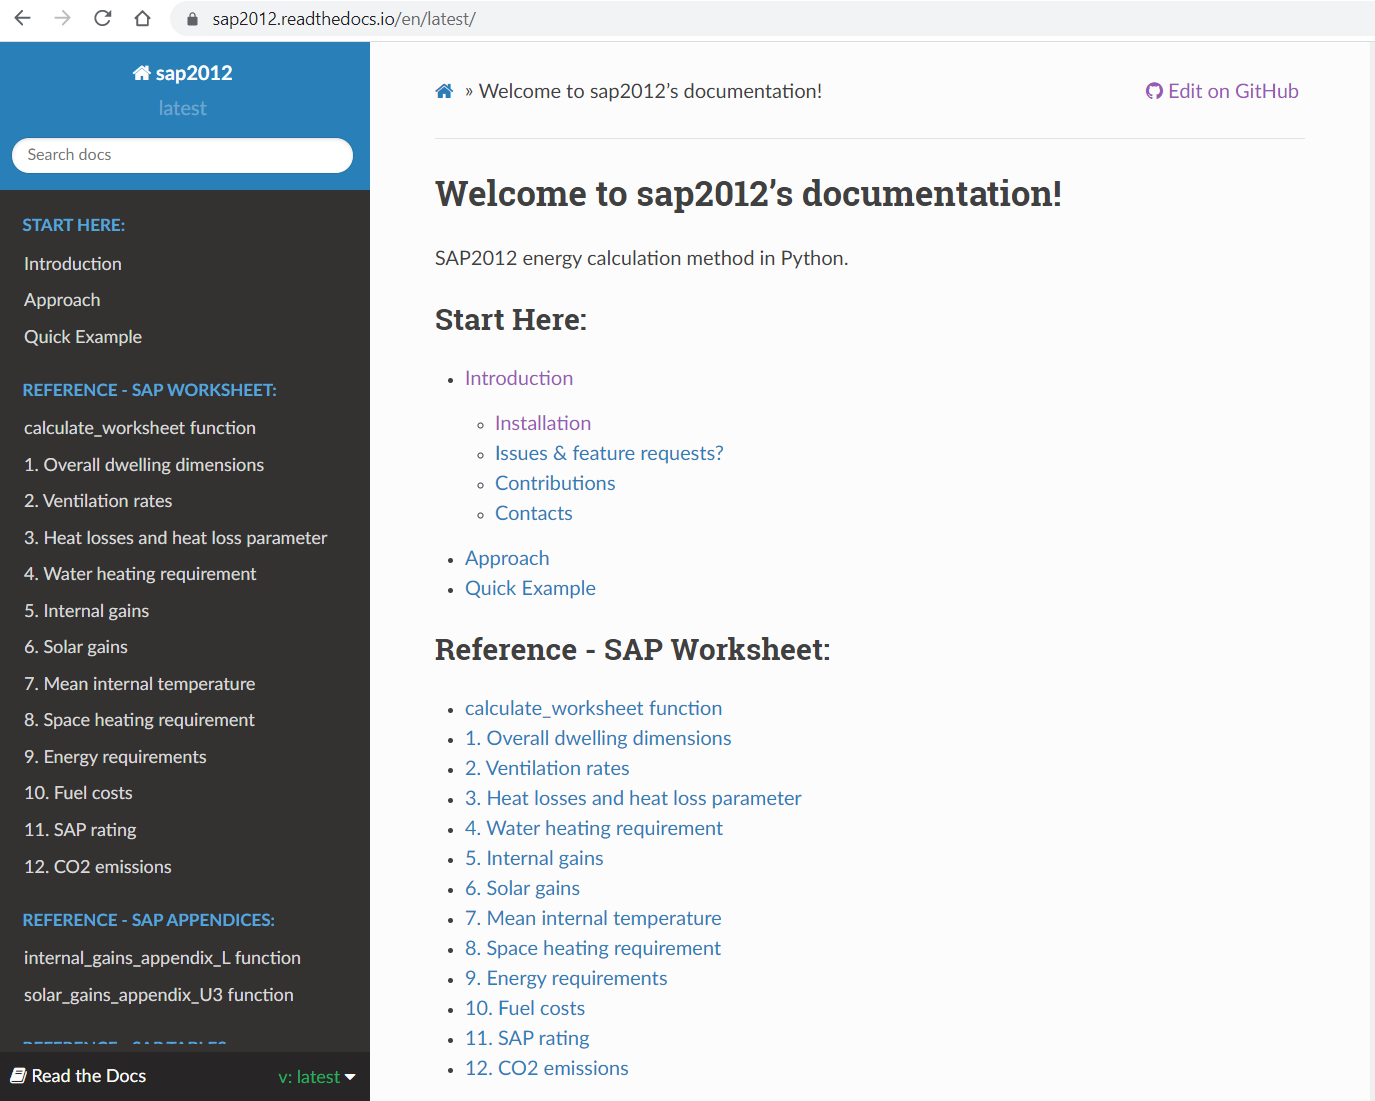
\includegraphics[width=0.9\textwidth,keepaspectratio]{readthedocs_sap_2012.png}
		\end{figure}
	\end{frame}


	\begin{frame}{A Python package for geometry calculations}

		\textit{crossproduct} - 2D and 3D geometry in Python.\\[10pt]
		
		This has classes relating to the major geometric objects:\\[10pt]

		\tikzstyle{every node}=[draw=black,thick,anchor=west,font=\footnotesize]
		\tikzstyle{description}=[draw=white]
		\tikzstyle{optional}=[dashed,fill=gray!20]
		
		\tikz \node {Point} [grow=right] child {node [description]{A 2D or 3D point, as described by xy or xyz coordinates}};
		\tikz \node {Vector} [grow=right] child {node [description]{A 2D or 3D vector, as described by xy or xyz coordinates}};
		\tikz \node {Line} [grow=right] child {node [description]{A 2D or 3D line, as described by a Point and a Vector}};
		\tikz \node {Halfline} [grow=right] child {node [description]{A 2D or 3D halfline, as described by a Point and a Vector}};
		\tikz \node {Segment} [grow=right] child {node [description]{A 2D or 3D segment, as described by two Points}};\\
		\tikz \node {Polyline} [grow=right] child {node [description]{A 2D or 3D polyline, as described by a series of Points}};
		\tikz \node {Plane} [grow=right] child {node [description]{A 3D plane, as described by a Point and a normal Vector}};
		\tikz \node {Polygon} [grow=right] child {node [description]{A 2D or 3D polygon, as described by a series of Points}};
		\tikz \node {SimplePolygon} [grow=right] child {node [description]{A 2D or 3D non-intersecting Polygon}};
		\tikz \node {Polyhedron} [grow=right] child {node [description]{A 3D polyhedron, as described by a series of Polygons}};
		
	\end{frame}

	\begin{frame}{A Python package for creating 3D BIM models}
	
		\textit{pybim} - The Python Building Information Modelling package\\[10pt]
		
		This has a series of linked classes similar to a gbXML file:\\[10pt]
		
		\tikzstyle{every node}=[draw=black,thick,anchor=west,font=\footnotesize]
		\tikzstyle{geometry}=[draw=black,fill=gray!20]
		\tikzstyle{optional}=[dashed,fill=gray!20]
		\begin{tikzpicture}[%
			grow via three points={one child at (0.5,-0.6) and
			two children at (0.5,-0.6) and (0.5,-1.2)},
			edge from parent path={(\tikzparentnode.south) |- (\tikzchildnode.west)}]
			\node {BIM}
				child { node {Campus}
					child { node {Building}
						child { node {Space}
							child { node [geometry]{ClosedShell}
								child { node [optional]{crossproduct.Polyhedron}
								}
							}
							child [missing] {}
							child { node {SpaceBoundary}
								child { node [geometry]{Polygon}
									child { node [optional]{crossproduct.SimplePolygon}
									}
								}
							}
						}
					child [missing] {}
					child [missing] {}
					child [missing] {}
					child { node {Surface}
						child { node [geometry]{Polygon}
							child { node [optional]{crossproduct.SimplePolygon}
							}
						}
					}
					}
			};
		\end{tikzpicture}
		
	\end{frame}



	
	\begin{frame}[fragile]
		\frametitle{Creating geometry using Python}
		\footnotesize
		\begin{lstlisting}[language=Python]
import pybim.gbxml601
bim = pybim.gbxml601.BIM(id='bim1')
campus = bim.add_campus(id='campus1')
building = campus.add_building(id='building1')
space = building.add_space(id='space1',
                           floor_polygon=((0.0, 4.0, 0.0),
                                          (4.0, 4.0, 0.0),
                                          (4.0, 0.0, 0.0),
                                          (0.0, 0.0, 0.0)),
                           extrud_vector=(0.0, 0.0, 3.0)
                           )
surface = campus.surfaces(space_inner='space1',
                          space_outer=None,
                          azimuth=180.0)[0]
opening = surface.add_opening(id='opening1',
                              polygon=((1.0, 1.0),
                                       (3.0, 1.0),
                                       (3.0, 2.0),
                                       (1.0, 2.0))
                              )
		\end{lstlisting}
		%\lstinputlisting[language=Python, numbers=left, xleftmargin=2em, frame=single, framexleftmargin=2em]{"C:/Users/cvskf/OneDrive - Loughborough University/_Git/stevenkfirth/PythonGeometryPaper/4_1_Case_Study_Single_Zone_with_Window/4_1_code.py"}
	\end{frame}

	\begin{frame}[fragile]
		\frametitle{Creating geometry using Python}
		\footnotesize
		\begin{lstlisting}[language=Python]
import matplotlib.pyplot as plt
fig = plt.figure(figsize=(10,8),dpi=300)
ax = fig.add_subplot(111, projection='3d')
bim.plot(ax)
		\end{lstlisting}
		\begin{figure}
			%\centering
			\includegraphics[width=0.7\textwidth,keepaspectratio]{"C:/Users/cvskf/OneDrive - Loughborough University/_Git/stevenkfirth/PythonGeometryPaper/4_1_Case_Study_Single_Zone_with_Window/Fig_4_1a".jpeg}
		\end{figure}
	\end{frame}


	\begin{frame}{Conclusions}
		\begin{enumerate}
			\item Reproducibility involves writing text-based commands, i.e. code, scripts, programming etc.\\[10pt]
			\item Building simulation can be made reproducible by:
			\begin{itemize}
				\item Creating the models using programming code.
				\item Running the models in EnergyPlus.
				\item Analysing the results using programming code.\\[10pt]
			\end{itemize} 
			\item The challenge is the 3D geometry of the building model. \\[10pt]
			\item New open source libraries and packages are required $\rightarrow$ this is work in progress\ldots.\\[10pt]
			%\begin{itemize}
			%	\item Doing geometry calculations (i.e. 3D polygon intersection, 3D polyhedron intersection)
			%	\item Working with BIM models that contain geometric and non-geometric data (construction, internal gains etc.)
			%	\item Interfacing with standard building simulation file formats (gbXML, idf, epJSON)
			%\end{itemize} 
			\item Questions, comments, please contact me at: \texttt{s.k.firth@lboro.ac.uk}
		\end{enumerate}
	\end{frame}

	%\begin{frame}{What is "Reproducible"?}
	%	The Alan Turing Institute in its publication 'The Turing Way' defines reproducible research for data science as: \\ [10pt]
	%	\begin{quote}
	%		Work that can be independently recreated from the same data and the same code that the original team used. 
	%	\end{quote}
	%\end{frame}




	
\end{document}